\documentclass{article}
\usepackage[utf8]{inputenc}
\usepackage[swedish]{babel}
\usepackage{authblk}
\usepackage[sorting=none]{biblatex}
\addbibresource{sources.bib}
\usepackage{graphicx}
\usepackage[T1]{fontenc}
\usepackage{ae}
\usepackage{multirow}
\usepackage[table]{xcolor}
\usepackage{pgfgantt}
\usepackage{pdfpages}

\title{\textbf{Larmsystem med MD407}\\ 
\hspace{10cm}
\hrule
\hspace{10cm}
Implementation av rörelsesensor, avståndsmätare och simulerad dörrenhet på MD407-mikrodator}
    
\author{\\Alamin Alreda\\Sebastian Danckwardt\\Zaid Haj Ibrahim\\Isac Holm\\Edvin Svahn}

\date{\today}
    
%LÄÖGGG TILL: handledare, e-post adresser, sektion, datum för senaste revision
    
\begin{document}

\maketitle
\newpage
\tableofcontents
\newpage
\section*{Ordlista}
\begin{description}

\item[ACK-meddelande] \emph{acknowledgement message} är ett meddelande som skickas i respons till att ett meddelande har tagits emot väl.

\item[Buss] En \emph{buss} är en kommunikationsport som tillåter överföring av data i form av elektriska signaler.

\item[CAN] \emph{Controller Area Network} är en databuss som tillåter kommunikation mellan mikrokontrollers. MD407 är försedd med två CAN bussar.

\item[GPIO] \emph{General Purpose Input/Output} är en anslutningsport på MD407 där olika logiska enheter kan anslutas för att ta emot eller skicka data.

\item[HC-SR04] En ultraljudsbaserad avståndsmätare.

\item[Knappsats] En extern periferienhet med 16 knappar som används för inmatning av data till mikrokontroller.

\item[SW-18010] En fjäderbaserad vibrationssensor.

\item[USART] \emph{Universal Synchronous/Asynchronous Reciever/Transmitter} är hårdvara som tillåter seriell kommunikation mellan mikrokontroller och PC.

\end{description}
 \newpage

\setcounter{page}{1}
\section{Introduktion}

Under året 2021 anmäldes 72 884 inbrottsstölder i Sverige vilket pekar på att det finns ett tydligt behov av larmsystem i dagens samhälle \cite{BRa}.
Trots den oro som finns i allmänheten för att ens egendom ska bli stulen så tillkännager endast 13 \% av unga mellan 23 och 35 år att de äger en larminstallation \cite{MoFor}.
En av de största anledningarna till detta är kostnaden, 20 \% av de som saknar ett hemlarm anger att priset på installation är för högt \cite{MoFor}.
Genom att skapa ett prisvärt larmsystem kan man erbjuda möjligheten till en tryggare tillvaro.

%NY INTRODUKTION ADDERAD

\subsection{Syfte}
Projektet syftar till att skapa ett kostnadseffektivt larmsystem som är lätt att använda.
Detta då endast 29 \% av Sveriges befolkning äger ett larmsystem \cite{SSF}.
Systemet är menat installeras i bostäder, vilket kommer att sänka inbrott samt öka trygghet i framförallt låg-inkomsthushåll.
För att larmsystemet ska fungera säkert och korrekt, måste mål sättas upp. 

%ÄNDRA: sista meningen skum ändra från "eventuellt att kunna installeras"

\subsection{Mål}
Målet med projektet är att konstruera ett larm och låssystem med två periferienheter.
Den ena ska kunna upptäcka i fall en dörr står öppen, och den andra ska detektera om någonting rör sig inom en viss zon samt vibrationer i exempelvis ett fönster. 
Ett delmål är att ha en central styrenhet som ska utgöra den del av larmsystemet som har i uppgift att kommunicera med de perifera larmenheterna, den ska även kunna upptäcka ifall en periferienhet har kopplats bort från systemet.
Målet med detta är att möjliggöra centraliserad kontroll och kalibrering av flera larmenheter i ett larmsystem.
Ytterligare ett delmål är att ha en enhet som ska agera defekt för att kunna testa ifall systemets kommunikation är robust nog för att hantera överflöd av data.

\noindent
\\
Ett delmål med lägre prioritet är att centralenheten ska kunna konfigurera en ny periferienhet vid anslutning. När den centrala styrenheten startar ska en förfråga skickas till de anslutna periferienheterna. 
Därpå svarar varje periferienhet med dess typ och konfiguration för att sedan tilldelas ett unikt ID. 
Dörrenhetens mål är att inledningsvis larma lokalt med en röd lysdiod. 
Dörrlarmet larmar till centralenheten efter att det lokala larmet har varit igång under en specifik kalibreringsbar tid vilket kan sättas av användaren. Till exempel 4 sekunder till lokala larmet att slås på och 8 sekunder till centrala larmet.
Avståndsmätare ska larma centralt ifall något passerar framför den inom ett visst avståndsintervall, ett delmål med lägre prioritet är att även implementera ett lokalt larm för avståndsmätaren.
Vibrationssensorn ska detektera rörelse i form av vibrationer som antingen kan färdas i luften eller genom materialet som den är fäst vid. 
Ett centralt mål ska vara att låsa eller låsa upp dörren samt inaktivera dörrlarmet genom att mata in en fyrsiffrig kod på en knappsats ansluten till centralenheten.

%ÄNDRA: gör tydligt vad som är delmålen i projektet

\subsection{Arbetsmetod}
I arbetsmetod beskrivs hur gruppen har jobbat. Det finns 3 stora delar som har bidragit till den färdiga produkten. Förarbetet som gav en klarare bild av hur arbetet skulle utföras. Hur tekniska genomförandet gick till sedan testning och verifiering av kod för att undvika buggar och svagheter i systemet.

\subsubsection{Förarbete}
Innan kod skrevs behövdes genomförandet av projektet planeras. 
Detta inkluderar bestämning av versionskontroll system, kommunikationsplatform, testning av produkten samt ordning av larmsystemets olika delar. 
Versionskontrollsystemet som valdes var Github, kommunikationsplatform valdes Discord. 
För att testa systemet gjordes en testmall för hur ett test skulle genomföras. 
Ordning av projektets olika delar gjordes genom en planering av olika milstolpar, först lades stort fokus på pereferienheterna, endast när dessa närmade sin slutpunkt skulle fokuset skifta till CAN protokollet för att kommunicera mellan dem. 
Motivationen till detta var att CAN protokollet inte skulle behövas förrän pereferienheterna var klara och att jobba på de enheterna skulle ge en klarare bild över hur CAN protokollet skulle fungera som effektivast.

\subsubsection{Tekniskt genomförande}
När kod började skrivas delades projektet upp i tre delar som arbetades på parallellt med varandra.
När en del var klar försökte de hjälpa de andra att komma ikapp tills alla var klara med sin del.
Sedan gick gruppen igenom vad som var kvar och delegerade arbetet. 
I början var gruppen inte helt bekväm med kommunikationsmediet vilket förvärrades av att alla i gruppen inte var på plats vilket ledde till att det producerades två versioner av avståndsmätaren.
Detta löstes genom att en ny version skapades från de bästa delarna av dem.
Efter dessa delar var klara gjordes CAN protokollet medans buggar fixades i pereferienheterna. Centralenheten gjordes i samband med CAN protokollet då centralenhetens jobb inte kunde utföras utan en fungerande kommunikationsmodell.
Efter detta gjordes störenheten för att simulera en defekt enhet.

\subsubsection{Testning och verifiering}
För att säkerställa kvalitén hos producerad kod testades färdig kod kontinuerligt med under arbetsprocessen med testmallar.
Rent praktiskt var ofta olika print-statements placerade i koden för att kolla så att korrekt resultat producerades i kombination med att sätta objekt framför avståndsmätare, osv.
Då inget fel noterades var testet markerat som godkänt och ingen vidare åtgärd tillämpades. 
Däremot när resultat inte blev som testet förväntat söktes felkälla upp och fixades omgående, sedan gjordes ett nytt test för att säkerställa fungerande produkt. 
Utöver att testa kodens vanliga funktion har den testas mot olika typer av angrepp med hjälp en störenhet som skickar data för att störa centralenhetens normala funktion. 
Detta genom att  skicka stora volymer data. 
Störenheten användes också som en angreppsenhet, med hjälp av den så testades centralenhetens motstånd mot återuppspelningsattacker samt imitationsattacker.

\section{Teknisk beskrivning}
I det här kapitlet redogörs en teknisk beskrivning av systemet. 
I den tekniska bakgrunden beskrivs vad samtliga komponenter har för syfte. Därefter ger Systemöversikt en övergripande förståelse för hur systemet är uppbyggt. 
Delsystem förklarar hur samtliga delarna är uppbyggda.

\subsection{Teknisk bakgrund}
Larmsystem kan ha olika konstruktion beroende på säkerhetsbehov men samtliga system tillämpar flertal olika sensorer för att upptäcka inbrott. 
I fall en avvikelse upptäcks av en sensor ska larmet aktiverats och användare underrättas.
\\
\\
I konstruktionsarbetet är MD407-mikrodator den centrala komponenten. 
Detta är en laborationsdator med stabil hårdvara som har utvecklats i utbildningssyfte. 
Då datorn är utvecklad för utbildning finns det skydd mot elektrostatiska urladdningar, felkopplingar och mekaniska påfrestningar vilket gör den lämpad för utveckling av prototypsystem.
\\
\\
För att MD407-mikrodator ska kunna skicka och ta emot data från externa perifierienheter är den försedd med flera olika anslutningar som kan användas för detta. 
GPIO lämpar sig för koppling med enklare periferienheter och är den anslutningen som används för kommunikation med avståndsmätare samt Vibrationssensor. 
Det finns 5 GPIO portar benämnda A-E. portarna har 16 kontaktstift vardera som kan konfigureras till att hantera indata eller utdata. 
Det finns även kontaktstift för ström samt jord som används av sensorerna.
\\
\\
Då åtskilliga MD407-mikrodator behöver kommunicera med varandra är de försedda med två CAN portar. Den sista anslutningen som används är USART, den används för att upprätthålla seriell kommunikation mellan en mikrodator och en PC.

\newpage
\subsection{Systemöversikt}

\\
\\
\noindent
Systemet i sin helhet består av tre delar, en centralenhet, en dörrenhet och en sensorenhet. Utöver dessa enheterna innehåller systemet övriga komponenter som bidrar till funktionalitet av systemet. Ett exempel på det kan vara knappsatsen.Ett av korten används som centralenhet som de övriga korten samt komponenterna kopplas till (figur 1). Kommunikation mellan samtliga MD407-mikrodator sker via en CAN-buss, medan kommunikation mellan centralenheten och PC sker över USART.
\\
\begin{figure}[h]
    \centering
    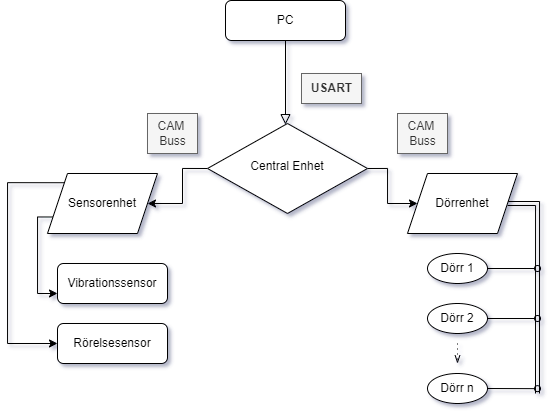
\includegraphics[scale=0.6]{Projektrapport/diagram.png}
     \caption {Blockschema av larmsystemet. Pilarna indikerar på GPIO-port koppling mellan dörrarna/sensorerna till kortet. Dubbel-pilar mellan dörenheten och dörrarna indikerar på att det finns en kopplingsplatta.}
    \label{fig:drawing}
\end{figure}
\newpage
\\
\noindent
Dörrenhet ska vara ansluten till en kopplingsplatta, på plattan ska det finnas lysdioder och möjlighet till att läsa av i fall dörren är öppen respektive stängd.
Lysdioderna kommer lysa rött när dörrenheten larmar lokalt eller grönt om inget larm har gått.
\\
\\
Till sensorenheten kopplas avståndsmätare (HC-SR04) och vibrationssensor (SW-18010P).
Avståndsmätaren kommer att skicka en signal om det avmätta avståndet ligger inom ett visst tröskelvärde.
På samma sätt kommer vibrationssensorn skicka en signal om den har känt av några vibrationer över ett tröskelvärde.

\subsection{Delsystem}
Här beskrivs vad de olika delsystemen har för tekniska funktioner samt vilket syfte de uppfyller i systemet.

\begin{figure}[h]
    \centering
    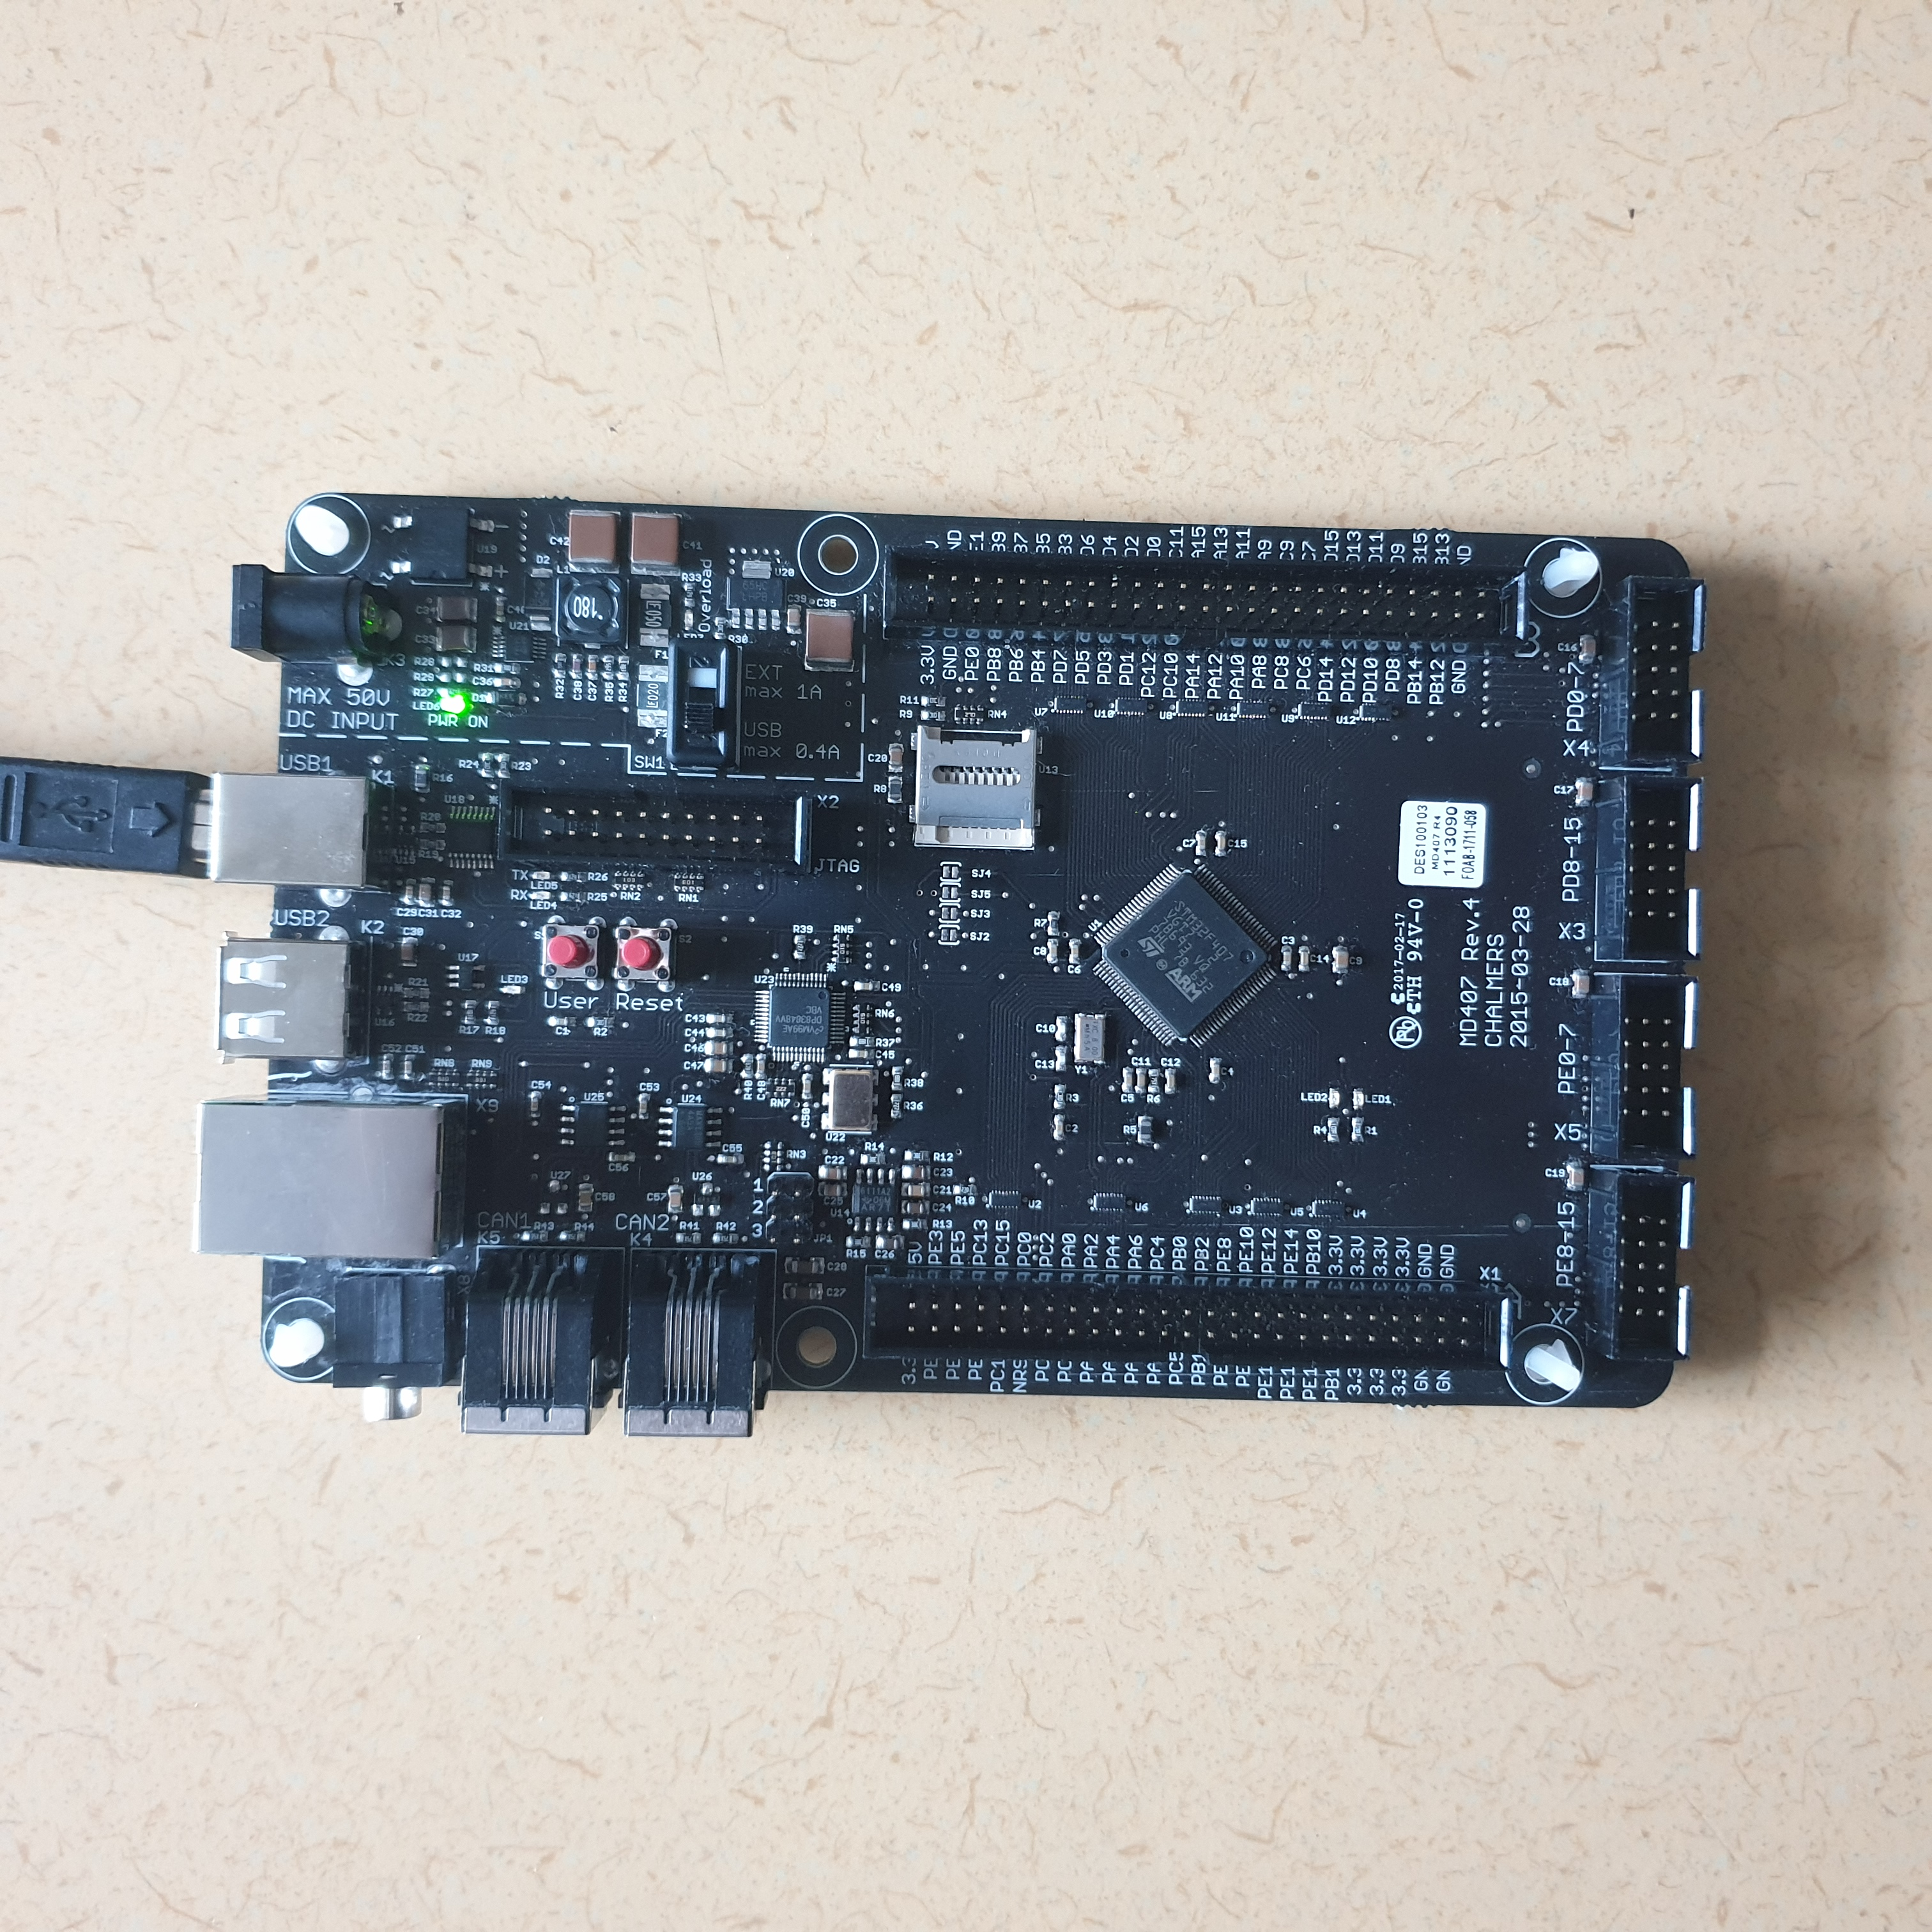
\includegraphics[scale=0.05]{Projektrapport/central.png}
    \caption {Hårdvaran som har funktionen som centralenhet}
    \label{fig:drawing}
\end{figure}

\subsubsection{Centralenhet}
Centralenheten är systemets hjärna. Dess huvuduppgift är att upprätthålla en konstant kommunikation mellan sig själv och de anslutna enheterna. Centralenheten tar emot livstecken från anslutna enheter varje 500 millisekunder för att se till att enheterna fortfarande är anslutna. Ett larm utlöses om 1000 millisekunder passerar utan att centralenheten tar emot ett livstecken från en ansluten enhet.

\noindent Centralenheten tar också hand om tilldelningen av ID till anslutna enheter. När en annan enhet startar skickar den ett "NEW ALIVE"-meddelande med sin typ till den centrala enheten. Den centrala enheten tar sedan emot detta meddelande och svarar med ett ID för enheten, som den börjar använda för all framtida kommunikation.

\noindent Dessutom sköter centralenheten all kommunikation mellan användaren och systemet via USART och en knappsats. När centralenheten startar uppmanar den användaren att ange ett lösenord. När det har angetts visar centralenheten sedan en meny med nio alternativ. Användaren kan då ändra lösenordet, uppdatera tröskelvärdet för varje dörr och sensorenhet, ändra tröskelvärdet för avståndsmätaren och se status för alla enheter som är anslutna till centralenheten.

\subsubsection{Dörrenhet}
En dörrenhet ansluts till flera dörrar, och dessa dörrar ansluts till ett lås och två lysdioder (en grön och en röd). Lysdioderna tänds beroende på den aktuella larmstatusen för varje dörr. Den gröna lampan tänds om det globala larmet är aktiverat, medans den röda lampan tänds om det lokala larmet är aktiverat. En ytterligare lysdiod är ansluten till dörren, som tänds eller släcks om dörren är låst eller olåst. Användaren kan välja att låsa en dörr genom att skicka ett meddelande från centralenheten. 



\subsubsection{Sensorenhet}

Sensorenheten kommer att vara kopplad till två sensorer: avståndsmätare och vibrationssensor (HC-SR04 respektive SW-18010P).
Avståndsmätaren kommer att läsa av avståndet till ett objekt genom att skicka ultraljudssignaler och vänta på att få tillbaka ett eko. 
Mätningen av avståndet kommer att ske genom att räkna skillnaden i mikrosekunder mellan ultraljudssignaler och deras eko, därefter divideras tiden med 58 för att få avståndet i centimeter. 
Avståndet kommer att mättas kontinuerligt i intervaller av 60 millisekunder, om avståndet överstiger eller blir mindre än tröskelvärdet kommer det centrala larmet att gå.\\
\\
Sedan kommer även vibrationssensor att känna av vibrationer, ifall den känner av någon vibration kommer den att meddela centralenheten för att aktivera det globala larmet.

\begin{figure}[!tbp]
    \centering
    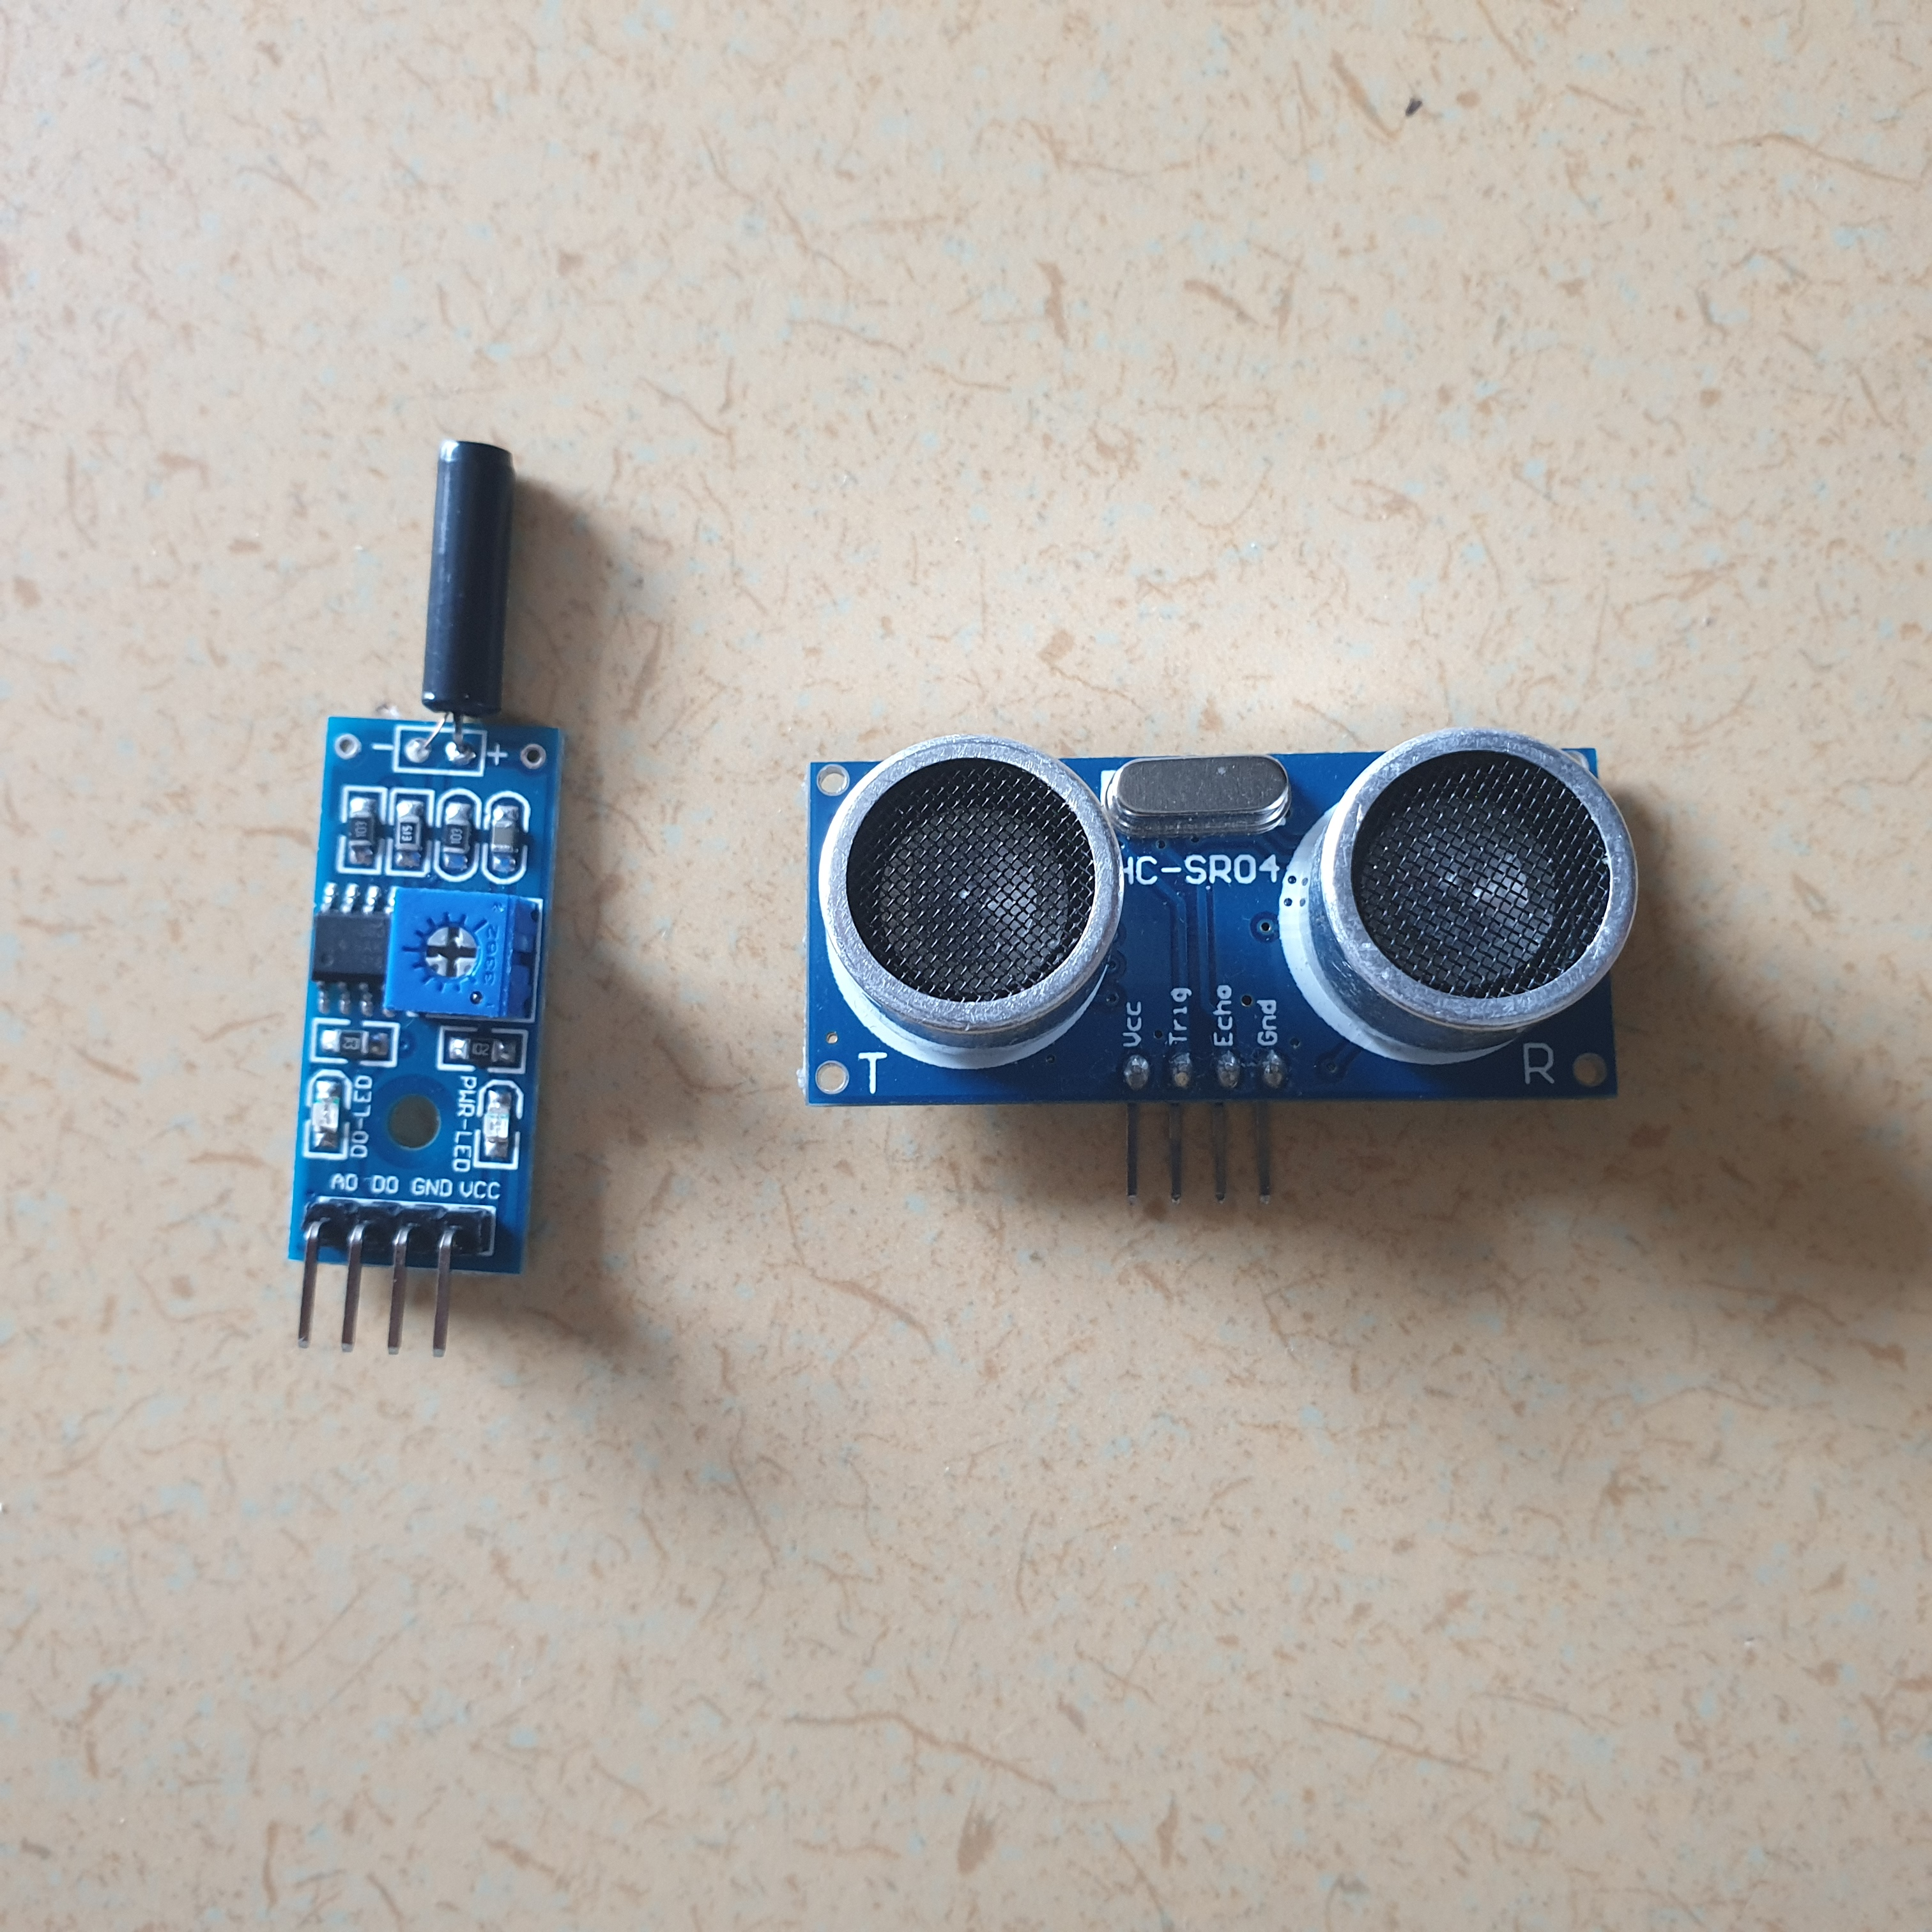
\includegraphics[scale=0.04]{Projektrapport/sensor.png}
    \caption {Sensorerna som är implementerade på sensorenheten. Hårdvaran till vänster är vibrationssensor och till höger är avståndsmätare}
    \label{fig:drawing}
\end{figure}


\subsubsection{Systemprotkoll}
Kommunikationsprotkollet är ett 11 bitar långt protokoll uppdelat i fyra segment (figur 2).
Den mest signifikanta biten är bit 10 och minst signifikanta biten är bit 0. 
Ettställning av bit 10 innebär att meddelandet får högsta prioritet när det tas emot på bussen ifall det redan finns meddelanden i bufferten.
Nollställning av samma bit innebär då motsatsen, vilket är att meddelandet får lägsta prioritet och kan därmed vänta med utförande. 
Bit 9 till och med bit 6 är reserverade för meddlandetypen som innehåller bland annat ifall meddelandet är en förfrågan att larma på eller av, eller information som skickas mellan enheterna regelbundet. 
Varje gång ett meddelande skickas, kommer bit 5 till och med bit 3 innehålla avsändarens ID, och bit 2 till och med bit 0 innehålla mottagarens ID.


\begin{tabular}{|c|l|c|}
    \hline
    Bitmönster & Meddelandetyp & Innehåll \\
    \hline
    0000 & START ALARM & ... / DörrID \\
    0001 & STOP ALARM & ... /DörrID \\
    0010 & UNLOCK DOOR & DörrID \\
    0011 & NEW ALIVE & Enhetstyp \\
    0100 & NEW ALIVE RESPONSE & Enhetstyp hos mottagare \\ 
    &&och nytt ID \\
    0101 & RESET UNIT & ... \\
    0110 & SET DOOR ALARM TIME THRESHOLD & Nytt tröskelvärde \\
    0111 & SENSOR DISTANCE THRESHOLD & Nytt tröskelvärde \\
    1000 & RECALIBRATE & ... \\
    1001 & LIFESIGN & ... \\
    1010 & ACK & ... \\
    1011 & VIEW STATUS & ... \\
    \hline
\end{tabular}
\\
\begin{center}
\caption{Figur 5: Bitmönster för de olika meddelandetyper som används för CAN-kommunikation. Meddelandetyper med lägre nummer har högre prioritet. "..."\ betyder att innehållet är tomt.}
\end{center}

\subsubsection{Installering av larmsystem}
Installationen av systemet bildar en hierarki där centralenheten och dörr- och sensorenhet är basenheter. Basenheterna består av olika delsystem. Centralenheten är hjärnan för hela sytemet. Dess huvudsaklig uppgift är att leda en kollektivt samarbete mellan alla enheterna. Detta innebär att utan centralenheten skulle larmsystemet inte fullgöra sitt syfte. 

\noindent Centralenheten kommunicerar med periferienheterna via CAN-protokoll som skickas över en RJ11 Telefonkabel som i sin tur är kopplade till CAN-porten i periferienhetens MD-kort. Därmed delsystem för CAN ska inkluderas i alla basenheterna. USB-koppling mellan OC och basenheterna är essentiellt för attt hålla USART-kommunikation och försörja enheterna med ström. Detta dessutom möjliggöra att ladda enhetensmjuksystem till sammanhörande MD-kort. Delsystemet för timer genererar en avbrott och används för tidställning i övrgia funktioner, och för att se till att livstecken på kopplade periferienhetern inte överskrider tidgränsen. Centralenheten använder sig av en delenhet som abstraherar funkionalitet av knappsatsen. Knappstasten är kopplade till centralenheten via GPIO portar.


\begin{figure}[h]
    \centering
    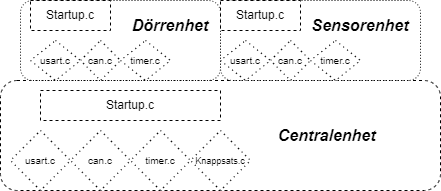
\includegraphics[scale=0.5]{Projektrapport/hierarki.png}
    \caption {Överblick av bildning av hierarki i larmsystemet. Varje basenhet innehåller en startup fil med enhetens huvudlogik. Övriga filer innehåller funktioner som bidrar till basenheterna}
    \label{fig:drawing}
\end{figure}


\section{Metod}

\subsection{Centralenhet}

\subsection{Dörrenhet}

Varje dörr har två tröskelvärden som bestämmer hur länge kan dörren vara öppnad innan ett lokalt respektive centralt larm slås på. Totalt definierades åtta dörrar för dörrenheten, till varje dörr delades fyra GPIO-pinnar. Första pinnen är en strömbrytare som kopplas direkt till 3,3 volt ström. Strömbrytaren kommer att anta värdet ett om dörren är stängd respektive värdet noll om dörren är öppen. Andra pinnen kopplas till en grön lampa som lyser när dörren är stängd eller släcks när dörren öppnas. Tredje pinnen kopplas till en röd lampa för att indikera ett lokalt larm. Lampan ska lysa när dörren har varit öppen för en bestämd tid, tiden bestäms genom centralenheten, och ska släckas när dörren är stängd. Sista pinnen kopplas till ett lås för att antigen låsa eller låsa upp dörren, vilket också görs genom centralenheten. Alla lampor kopplas upp på en kopplingsplatta enligt figur 7.
\\
\\Om en dörr öppnas startas en timer som utlöser ett larm när ett tidströskelvärde har uppnåtts. Denna tid beror på de tröskelvärden som ställs in av centralenheten. Som standard startar det lokala larmet fyra sekunder efter att en dörr har öppnats och det globala larmet startar åtta sekunder efter att det lokala larmet har utlösts. 

\begin{figure}[h]
    \centering
    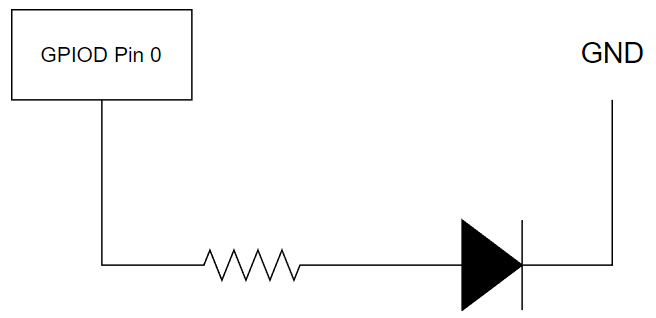
\includegraphics[scale=0.5]{Projektrapport/LED.png}
    \caption {Figuren visar hur en LED-lampa kopplas på en kopplingsplatta}
    \label{fig:drawing}
\end{figure}

\subsection{Sensorenhet}

Sensorenheten har två olika sensorer: en avståndsmätare och en vibrationssensor. Till avståndsmätaren delades två GPIO-pinnar. Första pinnen är trigg-pinnen och ansvarar för att skicka ultraljudspulser. Andra pinnen är eko-pinnen som antar värdet ett när ett eko kommer tillbaka och returnerar värdet noll om ingen läsning av eko sker. Skillnaden i tiden mellan när ultraljudspulsen skickades och när ekot har kommit tillbaka ges i mikrosekunder. Mätningen av avståndet sker enligt figur 8. Avståndsmätaren kopplas upp på en kopplingsplatta tillsammans med en röd lampa för att indikera att ett lokalt larm har inträffat. Trigg-pinnen sätts på för tio mikrosekunder innan den börjar vänta på eko-signaler. Hela mätningscykel sker i en intervall av 65 millisekunder. Sensorenheten kalibreras genom att en mätning utförs när det larmade området är tomt, för att få ett referensvärde. Referensvärdet används för att bestämma i vilka avstånds intervall ska enheten larma centralt respektive lokalt. Lokala larmet sker genom att tända den röda lampan medan centrala larmet skickar ett larm meddelande till centralenheten. Referensvärdet, intervallet för lokalt larm och intervallet för centralt larm kan ändras genom centralenheten.
\begin{figure}[h]
    \centering
    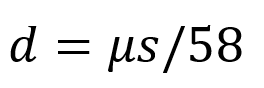
\includegraphics[scale=0.5]{Projektrapport/ekvation.png}
    \caption {Ekvationen ger avståndet i centimeter }
    \label{fig:drawing}
\end{figure}
\\
Vibrationssensorn har fyra pinnar: en ström-pinne, en jord-pinne, en digital output-pinne och en analog output-pinne. Under detta projekt har det bestämts att bara använda den digitala output-pinnen eftersom det finns bara behov av att läsa om en vibration har inträffats eller inte. Känsligheten för vibrationssensorn justeras med en komparator på själva sensorn. Sensorenheten skickar direkt ett alarm meddelande till centralenheten om en vibration har inträffats.

\subsection{Systemprotokoll}

\section{Resultat}
I detta avsnitt redovisas det för vad systemet kan göra och hur resultatet reflekterar de mål som sattes i projektets början. 
Det diskuteras även nackdelar med systemets konstruktion och vad som kunde ha gjorts på ett bättre sätt.

\subsection{Centralenhet}

\subsection{Periferienheter}
Ett centralt mål med projektet var periferienheterna som skulle ingå i systemet. 
Dörrenheten skulle upptäcka ifall en dörr står öppen och sensorenheten skulle upptäcka ifall något passerar framför den inom ett visst avståndsintervall samt rörelse i form av vibrationer.

\subsubsection{Dörrenhet}
Dörrenhetens implementation har uppnåt de delmål som sattes upp i början av projektet. 
Enheten kan hantera ett flertal dörrar, för varje enskild dörr kan tidsintervallen för aktivering av globalt respektive lokalt larm justeras individuellt med ett CAN-meddelande \emph{SET DOOR ALARM TIME THRESHOLD}. 
Den kan larma lokalt med en röd lysdiod i fall dörren är öppen och dess standard tidsintervall överskrids, efter tidsintervallet för globalt larm överskrids skickas ett CAN-meddelande \emph{START ALARM} till centralenheten.
Enheten kan skicka de periodvisa \emph{LIFESIGN} meddelanden som tas emot av centralenheten, den kan även avlarmas med ett \emph{STOP ALARM} meddelande.

\subsubsection{Sensorenhet}
Avståndsmätare gav förväntade resultat, genom testning och kalibrering med linjal kunde det verifieras att avståndsmätaren gav korrekt och konsekvent mätning av distans i cm.
Även om sensorn täcktes så att ekot inte registrerades kunde den larma vilket ökar säkerheten i systemet. 
Ett delmål med sensorenheten var att den likt dörrenheten skulle kunna larma både lokalt och globalt med avståndsmätaren. 
Avståndsintervallen för dessa kan konfigureras via ett CAN-meddelande \emph{SENSOR DISTANCE THRESHOLD} från centralenheten. 
Dock är intervallen inte individuellt reglerbara utan det är det lokala tidsintervallet som korrigeras till att bli det önskade intervallet medans det globala intervallet bestäms som en faktor av det lokala. 
Då enheten startar sätts intervallen till standardvärden som är bundna till den första mätningen av avstånd.
\\
\\
%Vibrationssensor, deaktivering av globalt larm

\subsection{Kommunikation via CAN och USART}

\subsection{Testning av system}
%simulering av defekt enhet överflöd idk

\section{Slutsats och diskussion}
Med resultaten kan man konstatera att det går att skapa ett eget larm som kan användas för bruk i bostäder.\\

\noindent
Den ena ska kunna upptäcka i fall en dörr står öppen, och den andra ska detektera om någonting rör sig inom en viss zon samt vibrationer i exempelvis ett fönster. 

\subsection{centralenhet}


\subsection{periferienheter}
\noindent
Dörrenheten 
\noindent
Eftersom att avståndsmätaren i nuläget bara jämför de värden som den får utan kontext och enskilt för varje mätning betyder det att det centrala larmet kan utlösas av att exempelvis en fluga flyger framför mätaren.
Det är ju så klart inte bra att ett hemlarm utlöses för att en fluga råkade flyga förbi mätaren, så om systemet skulle förbättras hade det varit smart att ändra på avståndsmätarens sätt att analysera sådant att den kanske måste få samma avstånd på flera gånger innan den börjar larma.\\

\noindent
Tyvärr så kan mycket problem uppstå ifall man väljer att skapa systemet själv.
För det första så måste man räkna med att få spendera mer tid för att programmera de olika delsystemen samt för att koppla ihop allting, för att inte tala om att bygga ett protokoll från grunden.
I fallet med kortet MD407 kan det bli begränsande vilka utvecklingsmiljöer som fungerar att använda felfritt då det inte finns så mycket dokumentation på just det kortet jämfört med kanske lite vanligare kort såsom en Arduino eller ett Raspberry Pi.\\

\noindent
Fördelarna väger fortfarande tungt då det både är billigare att köpa in de diverse komponenterna och koppla själv än att köpa en prenumeration där installation ingår, samt ger en större valmöjlighet när det kommer till egenskaper. 
Man kan till exempel använda sig av en motor som man kopplar en avståndsmätare på för att kunna få den att snurra runt sin axel och på så sätt kunna få en kamera som kan se runt sig och få en bild av omgivningen i form av avstånd.\\


\newpage
\begin{appendix}
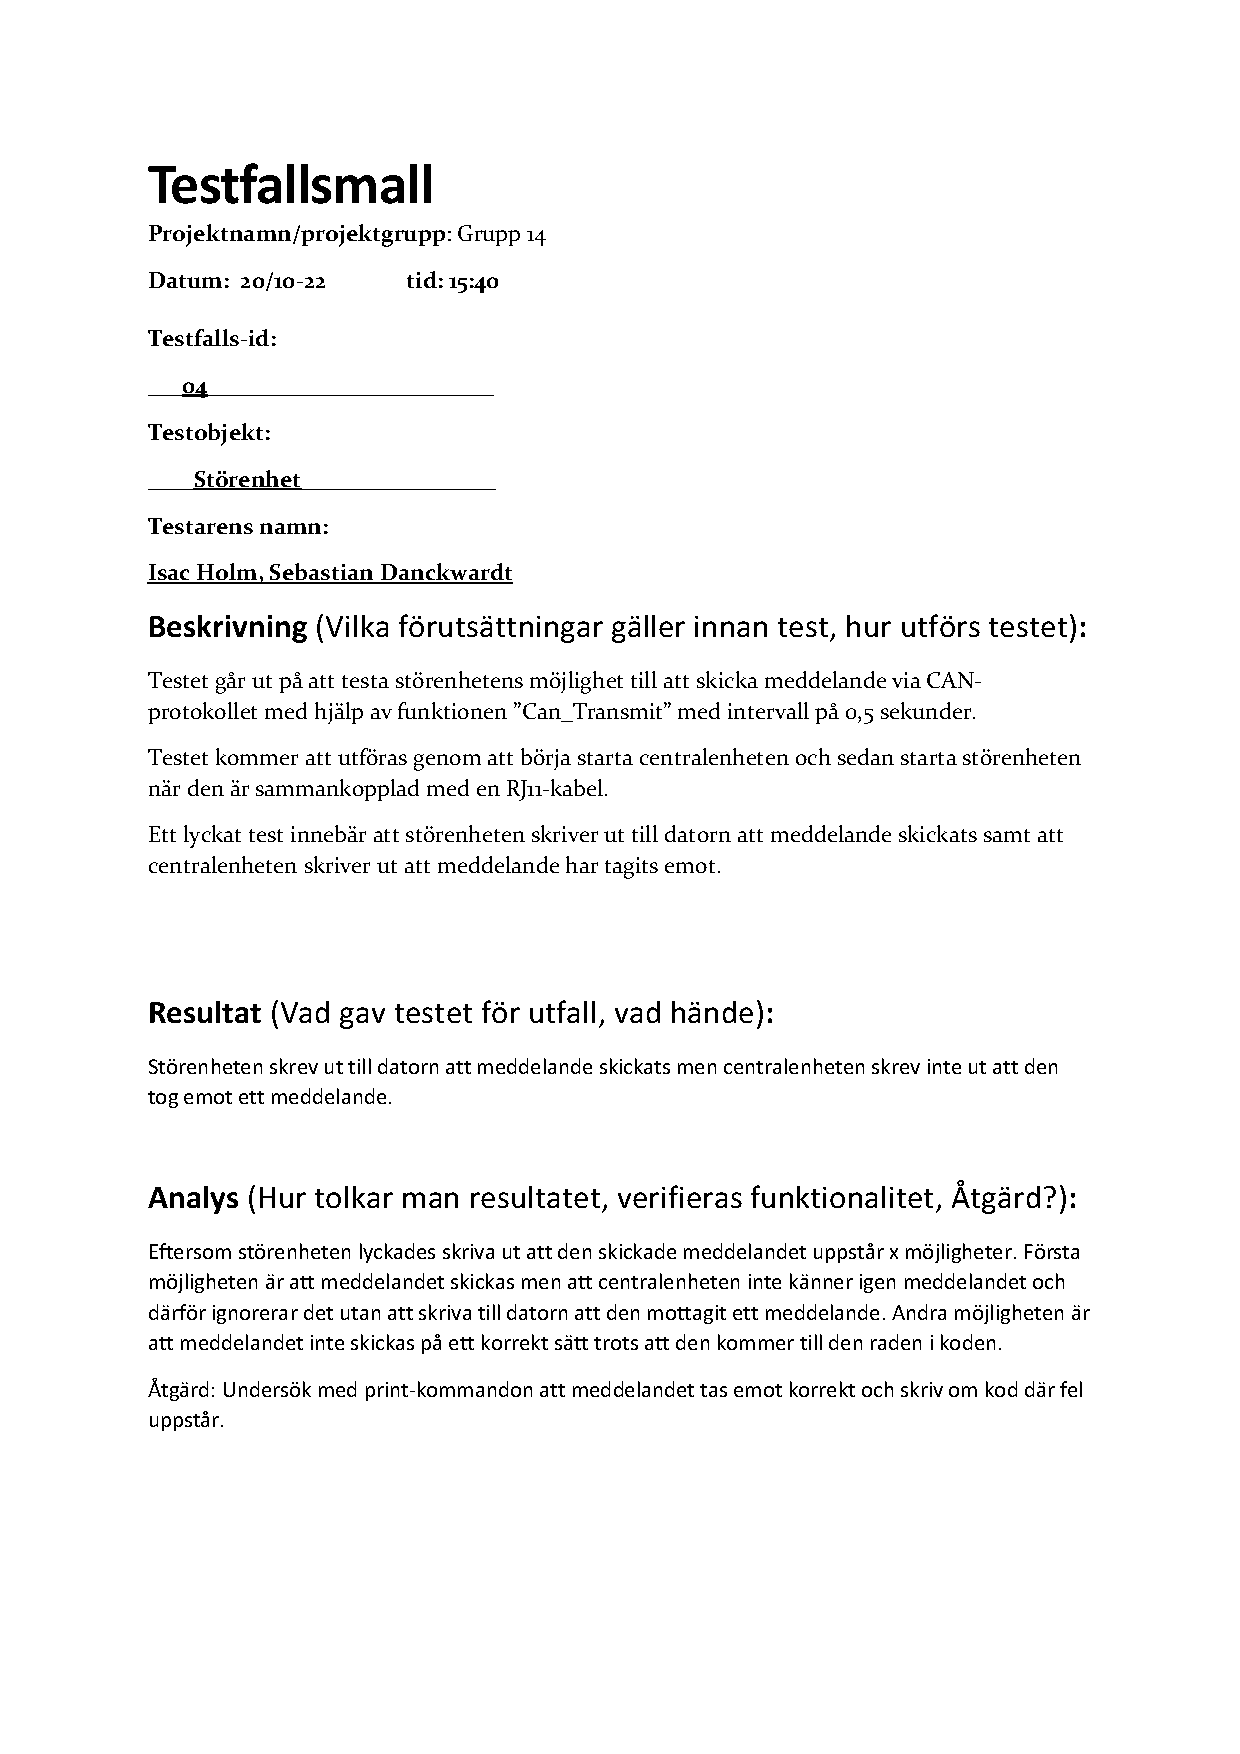
\includepdf[page=1, scale=0.8, pagecommand={\section{Testfall}}]{Testfallstorenhet.pdf}
\end{appendix}
\newpage

\section*{Källförteckning}
\printbibliography[heading=none]

\end{document}